%%%%%%%%%%%%%%%%%%%%%%
% SKYLINE COALESCENT METHODS
%%%%%%%%%%%%%%%%%%%%%%
\section{Phylodynamics}

\begin{frame}
\frametitle{Virus Phylodynamics}

%\center{
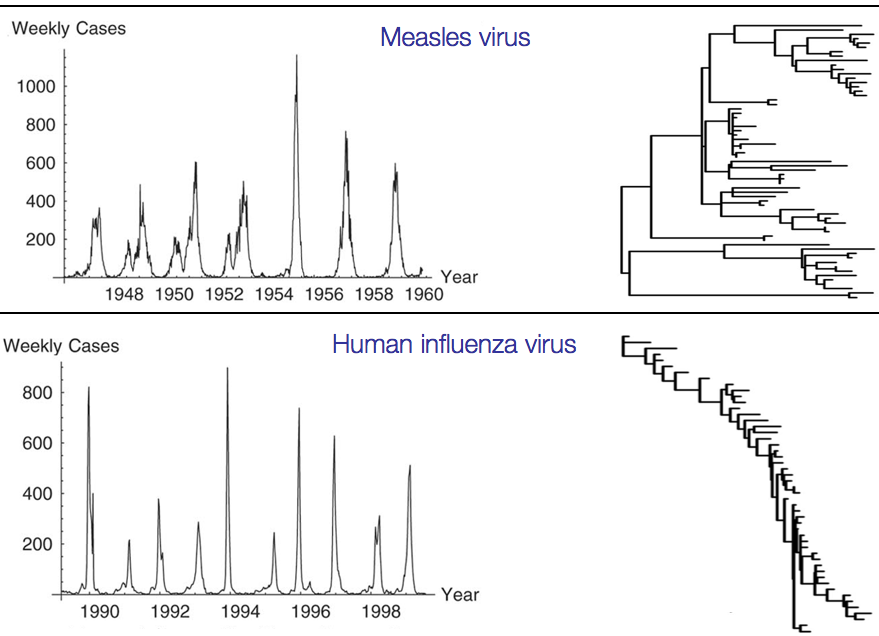
\includegraphics[scale=0.35]{../common/images/virusPhylodynamics}
%}
\end{frame}

\begin{frame}
\frametitle{``Skyline'' coalescent model}
\begin{centering}%
\pgfimage[width=0.8\textwidth]{../common/images/skylineModel}%
\par%
\end{centering}%
\end{frame}

\begin{frame}
\frametitle{The generalized skyline plot}

Introduced by Pybus and Strimmer (2001).

\begin{itemize}
\item Visual framework for exploring the demographic history of sampled DNA sequences
\item Input: a single estimated ancestral genealogy (a tree)
\item Output: nonparametric plot of the population size through time
\item Groups adjacent coalescent intervals 
\item Converts information within these intervals to estimates of population size
\end{itemize}

\medskip
\begin{columns}[t]

\column{0.5\textwidth}
for a single coalescent interval:

\begin{equation*}
\hat{N}_k = \binom{k}{2}t_k
\end{equation*}

\column{0.5\textwidth}
for $j$ adjacent intervals:
\begin{equation*}
\hat{N}_{k,j} = \frac{k(k-j)}{2j}\sum_{i=k-j+1}^k{t_i}
\end{equation*}

\end{columns}

\end{frame}

\begin{frame}
\frametitle{The generalized skyline plot - simulated data}

\begin{columns}[t]

\column{0.5\textwidth}
Constant population size, $N(t)=N_0$

\column{0.5\textwidth}
Exponential growth, $N(t) = N_0 e^{-rt}$

\end{columns}

\medskip

\begin{columns}[b]

\column{0.5\textwidth}

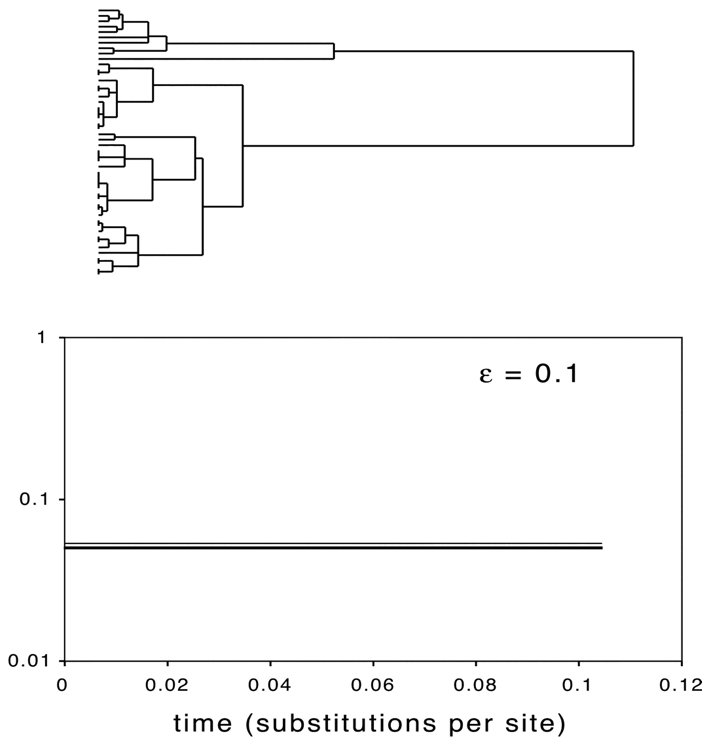
\includegraphics[scale=0.2]{../common/images/genSkylineConstant}

\column{0.5\textwidth}

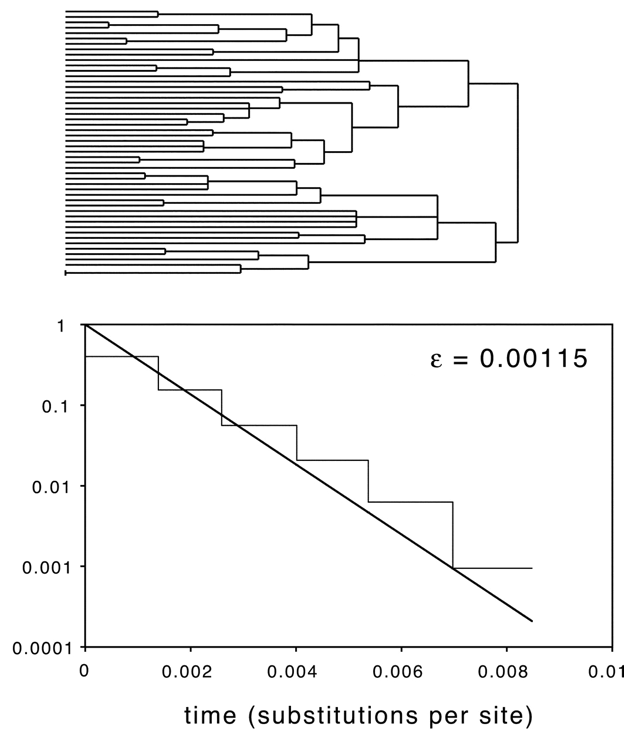
\includegraphics[scale=0.2]{../common/images/genSkylineExponential}

\end{columns}

\end{frame}

\begin{frame}
\frametitle{The generalized skyline plot - HIV-1 group M}


The tree used here was estimated in Yusim {\it et al} (2001) {\it Phil. Trans. Roy. Soc. Lond. B} {\bf 356}:855-866.

The black curve is a parametric coalescent estimate obtained from the same data under the expansion model, \small{$N(t) = (N_0-N_A)e^{-rt}+N_A$}

\bigskip

\begin{columns}[b]

\column{0.5\textwidth}

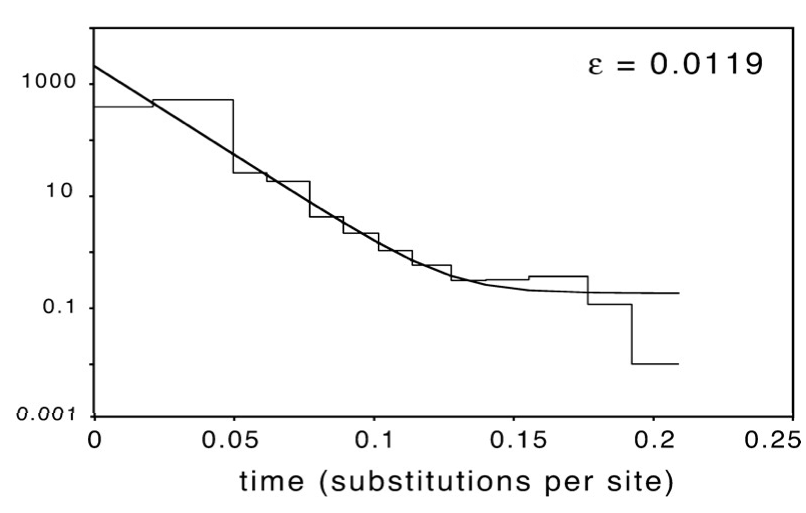
\includegraphics[scale=0.2]{../common/images/skylinePlotHIV}

\column{0.5\textwidth}

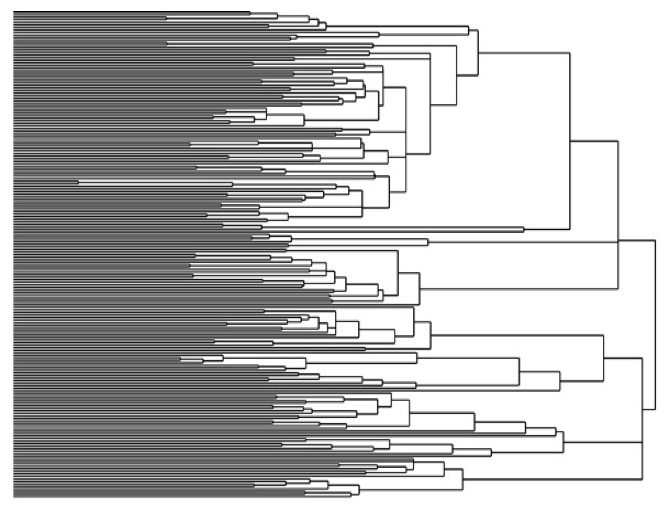
\includegraphics[scale=0.2]{../common/images/skylineTreeHIV}

\end{columns}

\end{frame}
